\documentclass[conference,a4paper]{IEEEtran}
\usepackage{amsmath}
\usepackage[ruled,vlined]{algorithm2e}
\usepackage{graphicx}
\usepackage{pifont}
\usepackage{textcomp}
\usepackage{xcolor}
\usepackage{tikz}
\usetikzlibrary{arrows.meta}
\usepackage{orcidlink}
\usepackage{subcaption}
\usepackage{makecell}
\usepackage[none]{hyphenat}
\usepackage{booktabs}
\usepackage{adjustbox}
\usepackage{longtable}
\usepackage{amssymb}
\usepackage{flushend}
\usepackage{pifont}
\usepackage{multirow}
\usepackage[protrusion=true,expansion=true]{microtype}
\usepackage{float}
\usepackage{comment}
\hypersetup{hidelinks}
\def\BibTeX{{\rm B\kern-.05em{\sc i\kern-.025em b}\kern-.08em
  T\kern-.1667em\lower.7ex\hbox{E}\kern-.125emX}}

\makeatletter
\newcommand{\linebreakand}{%
\end{@IEEEauthorhalign}
\hfill\mbox{}\par
\mbox{}\hfill\begin{@IEEEauthorhalign}
}
\makeatother

\begin{document}

\title{Platform-Aware Energy Modeling and Model-Symmetric Multi-Hub Route Screening for Delivery Drones
\thanks{\textit{\IEEEauthorrefmark{1} Corresponding author: Duc Ngoc Minh Dang (ducdnm2@fe.edu.vn)}}}

\author{%
\IEEEauthorblockN{
Trang Huyen Nguyen~\orcidlink{0009-0006-3490-2426},
Sang Tuyet Pham~\orcidlink{0009-0006-0777-7770},
Tan Thanh Nguyen~\orcidlink{0009-0000-0285-4403},
Khanh Vi Luu~\orcidlink{0009-0007-9166-7677},\\
Han Ho Ngoc Bui~\orcidlink{0009-0004-6630-045X},
Duc Ngoc Minh Dang\IEEEauthorrefmark{1}~\orcidlink{0000-0001-9302-3129}
}
\IEEEauthorblockA{
\textit{Faculty of Information Technology, FPT University}, Ho Chi Minh City, Vietnam\\
\{ntrang2110, sangpt050896,
captainparrot13042005, karlpro812005,
buihongochan.lodi\}@gmail.com, ducdnm2@fe.edu.vn
}}

% \author{
% \IEEEauthorblockN{Nguyen Huyen Trang}
% \IEEEauthorblockA{\textit{Faculty of Information Technology}\\
% \textit{FPT University}\\
% Ho Chi Minh City, Vietnam\\
% \href{mailto:ntrang2110@gmail.com}{[ntrang2110@gmail.com](mailto:ntrang2110@gmail.com)}}
% \and
% \IEEEauthorblockN{Pham Tuyet Sang}
% \IEEEauthorblockA{\textit{Faculty of Information Technology}\\
% \textit{FPT University}\\
% Ho Chi Minh City, Vietnam\\
% \href{mailto:sangpt050896@gmail.com}{[sangpt050896@gmail.com](mailto:sangpt050896@gmail.com)}}
% \and
% \IEEEauthorblockN{Nguyen Thanh Tan}
% \IEEEauthorblockA{\textit{Faculty of Information Technology}\\
% \textit{FPT University}\\
% Ho Chi Minh City, Vietnam\\
% \href{mailto:captainparrot13042005@gmail.com}{[captainparrot13042005@gmail.com](mailto:captainparrot13042005@gmail.com)}}
% \linebreakand
% \IEEEauthorblockN{Luu Vi Khanh}
% \IEEEauthorblockA{\textit{Faculty of Information Technology}\\
% \textit{FPT University}\\
% Ho Chi Minh City, Vietnam\\
% \href{mailto:karlpro812005@gmail.com}{[karlpro812005@gmail.com](mailto:karlpro812005@gmail.com)}}
% \and
% \IEEEauthorblockN{Bui Ho Ngoc Han}
% \IEEEauthorblockA{\textit{Faculty of Information Technology}\\
% \textit{FPT University}\\
% Ho Chi Minh City, Vietnam\\
% \href{mailto:buihongochan[.lodi@gmail.com](mailto:.lodi@gmail.com)}{[buihongochan.lodi@gmail.com](mailto:buihongochan.lodi@gmail.com)}}
% \and
% \IEEEauthorblockN{Duc Ngoc Minh Dang\IEEEauthorrefmark{1}~\orcidlink{0000-0001-9302-3129}}
% \IEEEauthorblockA{\textit{AiTA Lab,}\\
% \textit{Faculty of Information Technology}\\
% \textit{FPT University}\\
% Ho Chi Minh City, Vietnam\\
% \href{mailto:ducdnm2@fe.edu.vn}{ducdnm2@fe.edu.vn}}
% }


\maketitle

\begin{abstract}
Reliable energy-aware routing requires leakage-resistant prediction and a fair comparison between recorded and hypothetical paths. This study integrates operational telemetry from DJI Matrice 100 and vertical take-off and landing (VTOL) delivery flights with time- and location-associated weather observations. Flight-level regressors are evaluated using platform-aware grouped validation and untouched holdouts. The retained 11-feature DJI CatBoost model, using three operational and eight environmental predictors, achieves $R^2=0.9299$ and a weighted mean absolute percentage error (WMAPE) of $3.94\%$ on 48 holdout flights. The negative $R^2$ for VTOL flights, together with the platform-stratified audit, is consistent with substantial domain shift; the high pooled $R^2$ therefore does not imply reliable cross-platform prediction. SHapley Additive exPlanations (SHAP) and controlled ablation identify speed as the dominant predictive variable, while the tested weather summaries provide no measurable incremental value under the grouped-validation design. A separate flight-grouped XGBoost model predicts additive segment energy with mean cross-validated $R^2=0.9775$ and WMAPE $=3.94\%$ over 590 segments. Across 15 paired historical missions, the conservative final policy achieves a mean predicted distance-per-watt-hour improvement of $3.62\%$, accepting 14 hypothetical alternatives and retaining the historical path for one mission. Among the 14 accepted alternatives, the mean and median improvements are $3.88\%$ and $4.11\%$, respectively; however, all 14 consume more total predicted energy. The results support bounded multi-hub route screening in the DJI-derived topology, not minimum-energy routing or deployment-ready hub placement.
\end{abstract}

\begin{IEEEkeywords}
delivery drones, energy efficiency, domain shift, explainable machine learning, multi-hub route screening
\end{IEEEkeywords}

%%%%%%%%%%%%%%%%%%%%%%%%%%%%%%%%%%%%%%%%%%%%%%%%%%%%%%%%%%%%%%%%%%%%%%
\section{Introduction}
%%%%%%%%%%%%%%%%%%%%%%%%%%%%%%%%%%%%%%%%%%%%%%%%%%%%%%%%%%%%%%%%%%%%%%

\subsection{Background}
Battery energy limits the range and operational flexibility of delivery unmanned aerial vehicles (UAVs). Energy demand varies with airframe, payload, speed, altitude, wind, mission geometry, and the assumptions used to translate these variables into power or energy~\cite{rodrigues2021,stolaroff2018,zhang2021,choudhry2021}. Data-driven estimators can learn nonlinear relationships from synchronized flight logs, but prediction quality alone is not sufficient for route-level decision making. Validation must prevent related observations from crossing data partitions, model behavior must be interpreted within the represented platform domain, and route energy must be aggregated in physically meaningful units.

\subsection{Research Problem}
Energy-aware drone planning faces three related problems. First, telemetry records and derived segments are nested within flights, so random row-wise splitting can overstate generalization. Second, datasets containing multiple drone models can produce apparently strong pooled scores while failing within an individual platform. Third, route efficiency is a ratio of distance to energy, whereas total energy is additive; therefore, predicting or ranking segment efficiency directly is not sufficient for route evaluation.

\subsection{Research Gap}
Prior work has connected learned UAV energy models with risk assessment, recharging, charging-station design, shared-base routing, and predictive skyway planning~\cite{choudhry2021,alyassi2023,pinto2022,meskar2024,ren2026}. Weather-aware studies also report that wind representation can improve selected UAV energy targets~\cite{somanagoudar2025,pang2026}. The less explored evaluation problem is how to combine platform-aware validation, incremental feature assessment, additive segment-energy prediction, and a symmetric comparison between a recorded mission and hypothetical alternatives under the same model.

\subsection{Research Objectives and Contributions}
This work does not propose a new machine-learning algorithm, a new routing
algorithm, minimum-energy routing, or physical hub optimization. Instead, it
presents a validation-aware framework connecting empirical UAV energy
prediction to bounded route screening. The study addresses four research
questions:
\begin{itemize}
    \item \textbf{RQ1:} How do operational and environmental variables contribute to flight-level energy-efficiency prediction?
    \item \textbf{RQ2:} How does model performance vary across DJI, VTOL, and combined-platform domains, and what evidence indicates domain shift?
    \item \textbf{RQ3:} Which regression configurations provide the strongest validated performance for flight-level energy-efficiency and segment-energy prediction, respectively?
    \item \textbf{RQ4:} How can predicted segment energy support higher-EE route screening in a constrained multi-hub topology?
\end{itemize}

The main contributions are threefold. First, the study audits DJI-only, VTOL-only, and pooled regressors and shows why between-platform separation can inflate pooled $R^2$ while within-platform VTOL prediction fails. Second, it triangulates post-selection SHAP with grouped ablation to distinguish model attribution from validated predictive contribution. Third, it uses a separate segment-energy model so that predicted watt-hours are summed before route-level distance-per-Wh is calculated. Historical and hypothetical paths are then scored by the same frozen model, while total energy is reported separately from the selected efficiency objective.

%%%%%%%%%%%%%%%%%%%%%%%%%%%%%%%%%%%%%%%%%%%%%%%%%%%%%%%%%%%%%%%%%%%%%%
\section{Related Work}
%%%%%%%%%%%%%%%%%%%%%%%%%%%%%%%%%%%%%%%%%%%%%%%%%%%%%%%%%%%%%%%%%%%%%%

\subsection{UAV Energy Consumption Prediction}
UAV energy research includes physics-based estimation and data-driven prediction. Analytical studies show that payload, aircraft design, velocity, route geometry, and mission conditions materially influence energy use and range~\cite{stolaroff2018,zhang2021}. Flight-log datasets have enabled machine-learning approaches that estimate energy, voltage, state of charge, and related power variables directly from telemetry~\cite{rodrigues2021,dai2024}. Weather-aware approaches further incorporate atmospheric variables or aircraft-relative wind information~\cite{somanagoudar2025,pang2026}. These studies establish that energy prediction can benefit from operational and environmental information, but performance must be evaluated under a validation design consistent with flight-level independence.

\subsection{Explainable AI for Machine Learning}
Explainable machine learning has been applied to UAV power and energy prediction to identify influential features and improve model transparency~\cite{abdellatif2025,luo2025,lundberg2017}. SHAP provides additive model-attributed explanations, while ablation tests can evaluate how predictive performance changes when information is removed. However, these methods quantify predictive contribution rather than causal intervention effects; their interpretation depends on the fitted model and feature distribution~\cite{janzing2020,kumar2020,aas2021}.

\subsection{Research Gap Analysis}
Energy-aware routing is already an established area. Prior studies have integrated energy estimates with mission planning and recharging, intermediate charging stations, shared-base routing, and predictive delivery planning~\cite{alyassi2023,pinto2022,meskar2024,ren2026}. Accordingly, this paper does not claim a new routing algorithm or individual modeling novelty. Instead, it is positioned as an empirical, leakage-aware, and platform-aware energy-model evaluation connected to bounded route screening. The methodological gap lies in the disconnect between (i) energy prediction, (ii) platform/domain validation, and (iii) route-level decision making, with limited evidence on model-symmetric historical-versus-hypothetical route screening.

%%%%%%%%%%%%%%%%%%%%%%%%%%%%%%%%%%%%%%%%%%%%%%%%%%%%%%%%%%%%%%%%%%%%%%
\section{Methodology}
%%%%%%%%%%%%%%%%%%%%%%%%%%%%%%%%%%%%%%%%%%%%%%%%%%%%%%%%%%%%%%%%%%%%%%

\subsection{Overall Framework}
The proposed framework follows six stages: (1) process DJI and VTOL data
independently into a common analytical schema; (2) perform platform-aware
flight-level feature and model validation; (3) explain the selected DJI model
using SHAP and controlled ablation; (4) learn additive segment energy on the
retained DJI domain; (5) construct a constrained virtual multi-hub graph and
screen historical and hypothetical routes with the same frozen segment-energy
model; and (6) compare route-selection objectives and audit hub/topology robustness.

\subsection{Flight Telemetry Dataset}
The primary source is the DJI Matrice 100 package-delivery dataset of Rodrigues \emph{et al.}~\cite{rodrigues2021}, which reports 209 flights with synchronized position, inertial, wind, voltage, and current measurements at approximately 5~Hz. The ingested table available to the pipeline contained 207 flight identifiers; after quality-control exclusions, the analytical corpus contains 194 flight identifiers and 249,011 telemetry observations. A second public dataset contains 75 VTOL delivery flights; 68 remain after schema harmonization and quality control~\cite{booker2023}. VTOL data are used to diagnose cross-platform behavior and are excluded from the final route experiment.

\subsection{Data Preprocessing}
Telemetry is processed separately for each platform and then mapped to a common schema. Processing includes chronological ordering, quality checks, handling of invalid records, and preservation of flight identifiers. Three-dimensional segment distance is computed as the Euclidean combination of horizontal Haversine displacement and the absolute altitude difference. Electrical energy is reconstructed from voltage-current power and trapezoidal time integration. Weather observations are associated with flight time and location using the Open-Meteo resource~\cite{zippenfenig2023}.

\subsection{Feature Engineering}
The flight-level operational feature group contains commanded speed, altitude, and payload. Eight environmental summaries are considered: temperature, dew point, humidity, wind speed, wind gust, wind direction, precipitation, and pressure. The finalized DJI flight-level model uses all 11 predictors, while grouped ablation separately evaluates whether the environmental group adds predictive value. The segment model additionally uses segment distance and relative wind angle. Variables that directly reconstruct the flight-level EE target, including cumulative distance and consumed energy, are excluded from flight-level predictors. Flight energy efficiency is defined as
\begin{equation}
\mathrm{EE}=\frac{D}{E_{\mathrm{Wh}}}\quad [\mathrm{m/Wh}],
\end{equation}
where $D$ is traveled distance and $E_{\mathrm{Wh}}$ is reconstructed electrical energy. A separate target, \texttt{segment\_energy\_wh}, is used for routing because watt-hours are additive across graph edges whereas efficiency ratios are not.

\subsection{Machine Learning Models}
Ten regression families spanning linear, tree, bagging, and boosting approaches, including CatBoost, XGBoost, and LightGBM~\cite{catboost2018,xgboost2016,lightgbm2017}, are compared on identical grouped development folds. The final flight-level models reported for domain comparison are CatBoost for DJI, CatBoost for VTOL, and ElasticNet for the pooled case. For route evaluation, XGBoost is trained separately to predict segment energy in Wh. The segment model is selected by flight-grouped cross-validation and then frozen before route enumeration.

\subsection{Explainable AI}
SHAP is applied after model and feature-set selection to all 48 DJI holdout flights. Global mean absolute SHAP magnitude is used to rank predictive contributions. Controlled group ablation and leave-one-feature-out ablation are conducted on development folds with fixed CatBoost settings. These analyses are interpreted as predictive evidence rather than causal effects~\cite{lundberg2017,janzing2020,kumar2020,aas2021}.

\subsection{Virtual Multi-Hub Route Screening}
Historical DJI trajectories are converted into a constrained directed graph by sampling trajectory anchors and clustering nearby anchors into virtual intermediate nodes. In the baseline topology, a 200~m sampling interval and 15~m clustering radius produce 17 virtual nodes and 36 directed edges. The segment corpus contains 592 mapped segments, of which 590 valid segments from 194 flights are retained.

A flight-grouped XGBoost model predicts the energy cost $\hat{e}_k$ of each candidate edge. Route energy is obtained by summing predicted segment energy before calculating distance-normalized route efficiency:
\begin{equation}
\widehat{E}(r)=\sum_{k\in r}\hat{e}_k,
\qquad
\widehat{\mathrm{EE}}(r)=\frac{D(r)}{\widehat{E}(r)}.
\end{equation}
Summing Wh before forming the route ratio is essential because segment-level efficiency ratios are not additive.

\subsubsection{Request Layers and Candidate-Path Eligibility}
The routing experiment distinguishes two request layers. \texttt{HISTORICAL\_MISSION} requests preserve the recorded origin, destination, path sequence, operating conditions, and environmental context of each mission. These 15 missions support paired historical-versus-hypothetical route decisions. In contrast, \texttt{TOPOLOGY\_OD} requests enumerate eligible ordered origin-destination (OD) pairs in the constructed graph using one representative operating-condition profile. The 147 topology requests measure graph coverage and node-selection behavior and are not treated as independent observed flights.

A candidate path must connect the same origin and destination, contain at least one intermediate virtual hub, use no more than ten directed hops, and remain within 1.5 times the weighted shortest-path distance. Historical-mission candidates are additionally constrained to 1.5 times the recorded mission distance. A topology request is retained only when at least two feasible multi-hub paths exist.

The same frozen segment-energy model is applied to both the recorded historical path and hypothetical candidate paths under the corresponding request-level feature profile. The primary route comparison is therefore model-symmetric: the predicted EE of the recorded historical path is compared with the predicted EE of each candidate. The highest-EE admissible candidate is selected only when it improves upon this baseline; otherwise, the historical path is retained. Observed historical energy and EE are reserved for a supporting realism check.

\subsubsection{Route Decision Policies}
Five policies are evaluated on the same candidate sets. P0 is the recorded historical path scored by the frozen segment-energy model and serves as the symmetric baseline. P1 selects the shortest admissible path, P2 selects the path with minimum predicted energy, P3 selects the path with maximum predicted distance-normalized EE and is the proposed policy, and P4 uses a weighted multi-objective score to balance EE and total energy. For P4,
\begin{equation}
\begin{aligned}
S_{P4}(r) &= w_{EE}EE_{norm}(r)+w_E[1-E_{norm}(r)],\\
&\quad w_{EE}+w_E=1.
\end{aligned}
\end{equation}
with default weights $w_{EE}=w_E=0.5$. Normalization is performed within each request-level candidate set. Ties are resolved deterministically by higher score, lower predicted energy, higher EE, shorter distance, and path identifier.

\subsubsection{Hub-Dominance Audit and Topology Sensitivity}
To determine whether a frequently selected virtual hub is structurally necessary or merely energy-preferred, the routing graph is audited using node degree, weighted betweenness centrality, candidate-path participation, topology-wide availability, and recommendation frequency. The most frequently recommended node in the historical layer is removed, excluding cases in which it is an origin or destination, and route selection is repeated with the same frozen segment model. Routability loss, best-route agreement, and relative change in best predicted EE are reported.

One-factor-at-a-time sensitivity varies the graph-construction parameters around the 200~m anchor and 15~m clustering baseline. The anchor interval is tested at 150, 200, and 250~m with clustering fixed at 15~m; clustering radius is tested at 10, 15, and 20~m with the anchor interval fixed at 200~m. The segment-energy model remains frozen across configurations, and recommendation consistency is computed only for historical missions directly matched to the baseline.


% ============================================================
% Virtual Multi-Hub Route-Screening Schematic
% ============================================================
\begin{figure}[H]
\centering
\resizebox{0.96\columnwidth}{!}{%
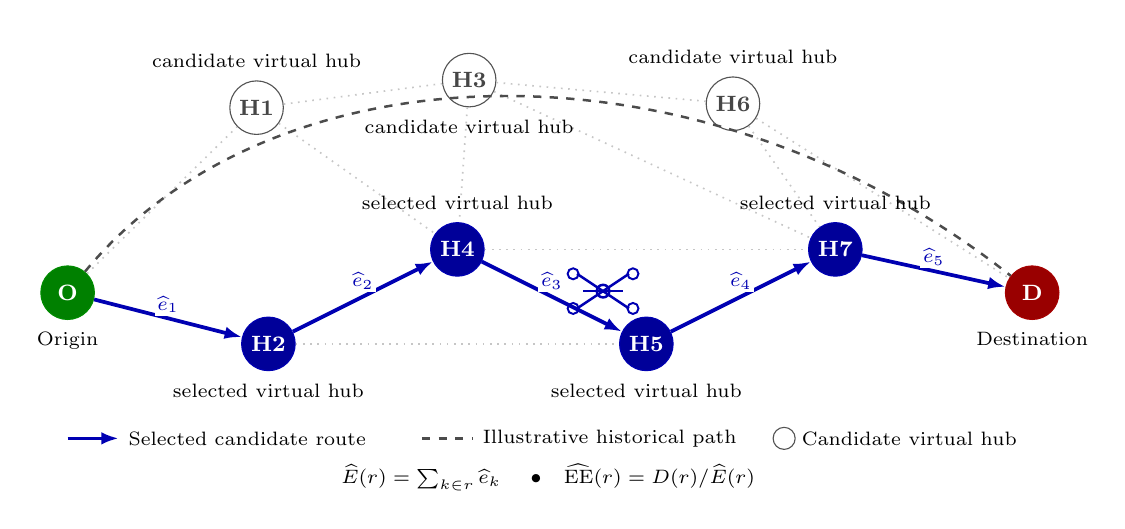
\begin{tikzpicture}[
    >=Latex,
    font=\scriptsize,
    selected/.style={
        circle,
        draw=blue!70!black,
        fill=blue!60!black,
        text=white,
        minimum size=0.68cm,
        inner sep=0pt,
        font=\footnotesize\bfseries
    },
    candidate/.style={
        circle,
        draw=gray!65!black,
        fill=white,
        text=gray!55!black,
        minimum size=0.68cm,
        inner sep=0pt,
        font=\footnotesize\bfseries
    },
    origin/.style={
        circle,
        draw=green!55!black,
        fill=green!50!black,
        text=white,
        minimum size=0.68cm,
        inner sep=0pt,
        font=\footnotesize\bfseries
    },
    destination/.style={
        circle,
        draw=red!65!black,
        fill=red!60!black,
        text=white,
        minimum size=0.68cm,
        inner sep=0pt,
        font=\footnotesize\bfseries
    },
    route/.style={
        -{Latex[length=2.2mm,width=1.6mm]},
        draw=blue!70!black,
        line width=1.35pt
    },
    historical/.style={
        dashed,
        draw=gray!60!black,
        line width=0.9pt
    },
    candidateedge/.style={
        dotted,
        draw=gray!45,
        line width=0.6pt
    }
]

% ============================================================
% NODES
% ============================================================

\node[origin] (O) at (0,0) {O};
\node[selected] (H2) at (2.55,-0.65) {H2};
\node[selected] (H4) at (4.95,0.55) {H4};
\node[selected] (H5) at (7.35,-0.65) {H5};
\node[selected] (H7) at (9.75,0.55) {H7};
\node[destination] (D) at (12.25,0) {D};

\node[candidate] (H1) at (2.40,2.35) {H1};
\node[candidate] (H3) at (5.10,2.70) {H3};
\node[candidate] (H6) at (8.45,2.40) {H6};

% ============================================================
% CANDIDATE CONNECTIVITY
% ============================================================

\draw[candidateedge] (O)--(H1);
\draw[candidateedge] (H1)--(H3);
\draw[candidateedge] (H3)--(H6);
\draw[candidateedge] (H6)--(D);

\draw[candidateedge] (H1)--(H4);
\draw[candidateedge] (H3)--(H4);
\draw[candidateedge] (H3)--(H7);
\draw[candidateedge] (H6)--(H7);

\draw[candidateedge] (H2)--(H4);
\draw[candidateedge] (H2)--(H5);
\draw[candidateedge] (H4)--(H7);
\draw[candidateedge] (H5)--(H7);

% ============================================================
% RECORDED HISTORICAL PATH
% ============================================================

\draw[historical]
    (O)
    .. controls (2.6,3.15) and (8.0,3.35) ..
    (D);

% ============================================================
% SELECTED ROUTE
% ============================================================

\draw[route] (O)--(H2);
\draw[route] (H2)--(H4);
\draw[route] (H4)--(H5);
\draw[route] (H5)--(H7);
\draw[route] (H7)--(D);

% ============================================================
% PREDICTED SEGMENT ENERGY
% ============================================================

\node[fill=white, inner sep=1pt, text=blue!70!black] at (1.275, -0.15) {$\widehat e_1$};
\node[fill=white, inner sep=1pt, text=blue!70!black] at (3.75,  0.15) {$\widehat e_2$};
\node[fill=white, inner sep=1pt, text=blue!70!black] at (6.15,  0.15) {$\widehat e_3$};
\node[fill=white, inner sep=1pt, text=blue!70!black] at (8.55,  0.15) {$\widehat e_4$};
\node[fill=white, inner sep=1pt, text=blue!70!black] at (11.0,  0.45) {$\widehat e_5$};

% ============================================================
% COMPACT NODE LABELS
% ============================================================

\node[anchor=north, yshift=-1pt] at (O.south) {Origin};
\node[anchor=north, yshift=-1pt] at (D.south) {Destination};
\node[anchor=north, yshift=-1pt] at (H2.south) {selected virtual hub};
\node[anchor=south, yshift=1pt]  at (H4.north) {selected virtual hub};
\node[anchor=north, yshift=-1pt] at (H5.south) {selected virtual hub};
\node[anchor=south, yshift=1pt]  at (H7.north) {selected virtual hub};
\node[anchor=south, yshift=1pt]  at (H1.north) {candidate virtual hub};
\node[anchor=north, yshift=-1pt] at (H3.south) {candidate virtual hub};
\node[anchor=south, yshift=1pt]  at (H6.north) {candidate virtual hub};
% ============================================================
% COMPACT DRONE ICON
% ============================================================

\draw[
    blue!70!black,
    line width=0.9pt
] (6.55,0.02)--(7.05,0.02);

\draw[
    blue!70!black,
    line width=0.9pt
] (6.80,0.02) circle (0.08);

\draw[
    blue!70!black,
    line width=0.9pt
] (6.80,0.02)--(6.47,0.24);

\draw[
    blue!70!black,
    line width=0.9pt
] (6.80,0.02)--(7.13,0.24);

\draw[
    blue!70!black,
    line width=0.9pt
] (6.80,0.02)--(6.47,-0.20);

\draw[
    blue!70!black,
    line width=0.9pt
] (6.80,0.02)--(7.13,-0.20);

\draw[
    blue!70!black,
    line width=0.7pt
] (6.42,0.24) circle (0.07);

\draw[
    blue!70!black,
    line width=0.7pt
] (7.18,0.24) circle (0.07);

\draw[
    blue!70!black,
    line width=0.7pt
] (6.42,-0.20) circle (0.07);

\draw[
    blue!70!black,
    line width=0.7pt
] (7.18,-0.20) circle (0.07);

% ============================================================
% COMPACT LEGEND
% ============================================================
\draw[route] (0.0,-1.85)--(0.65,-1.85);
\node[anchor=west] at (0.65,-1.85)
{Selected candidate route};
\draw[historical] (4.5,-1.85)--(5.15,-1.85);
\node[anchor=west] at (5.15,-1.85)
{Illustrative historical path};
\node[
    candidate,
    minimum size=0.28cm
] at (9.1,-1.85) {};
\node[anchor=west] at (9.2,-1.85)
{Candidate virtual hub};

% ============================================================
% FORMULA
% ============================================================

\node[
    align=center,
    font=\scriptsize
] at (6.15,-2.35)
{
$\widehat E(r)=\sum_{k\in r}\widehat e_k$
\quad$\bullet$\quad
$\widehat{\mathrm{EE}}(r)=D(r)/\widehat E(r)$
};

\end{tikzpicture}%
}

\vspace{1mm}

\caption{Schematic of constrained virtual multi-hub route screening. The UAV
moves from origin $O$ to destination $D$ through selected virtual hubs; each
directed segment receives a predicted energy cost $\widehat e_k$. Predicted
segment energies are summed before route-level energy efficiency is computed.
Virtual hubs are analytical graph nodes derived from historical trajectories
and do not represent physical facility locations.}
\label{fig:multi_hub_schematic}

\end{figure}

\section{Experimental Setup}

\subsection{Experimental Configuration}
Experiments use a fixed random state of 42 where applicable. Flight-level cases are evaluated separately for DJI, VTOL, and combined domains, while the routing branch uses the retained DJI domain. Route policies are evaluated on the same 15 historical missions and identical candidate sets. Five graph configurations are evaluated for topology robustness.

Table~\ref{tab:protocol} summarizes the datasets and evaluation protocols
used in the experiments.

\begin{table}[H]
\caption{Datasets and Evaluation Protocol}
\label{tab:protocol}
\centering
\scriptsize
\setlength{\tabcolsep}{2.5pt}
\begin{tabular}{p{0.24\columnwidth}p{0.31\columnwidth}p{0.35\columnwidth}}
\toprule
Task & Development & Final evaluation \\
\midrule
DJI flight EE & 146 flights; date-grouped cross-validation (CV)
& 48-flight untouched holdout \\
VTOL flight EE & 41 flights; date-grouped CV
& 27-flight diagnostic holdout \\
Combined flight EE & 199 flights; platform-date CV
& 63-flight pooled/stratified holdout \\
DJI segment energy & 590 segments from 194 flights
& 5-fold CV grouped by \texttt{flight\_uid} \\
\bottomrule
\end{tabular}
\end{table}

\subsection{Evaluation Metrics}
Flight-level performance is assessed with $R^2$, MAE, RMSE, median absolute error, signed bias, and WMAPE. For route screening, the primary comparison uses predicted historical and predicted candidate EE under the same frozen model. Total-energy saving is reported separately:
\begin{equation}
S_E=\frac{\widehat{E}_{\mathrm{hist}}-\widehat{E}_{\mathrm{rec}}}{\widehat{E}_{\mathrm{hist}}}\times100\%.
\end{equation}
Observed historical distance, energy, and EE are retained only as a supporting realism check and are excluded from the primary recommendation rule.

\subsection{Training and Validation Strategy}
Development and holdout partitions are created before feature or model comparison. DJI and VTOL flight-level development folds are grouped by acquisition date; the pooled case uses platform-date groups. Segment-energy folds are grouped by source \texttt{flight\_uid}. The chosen feature set, model family, and hyperparameters are fixed before the untouched holdout is opened. SHAP and ablation are conducted only after model selection. Route policies use the same frozen XGBoost model and the same candidate set for each request.

\section{Results and Discussion}

\subsection{Prediction Performance Comparison}
On the DJI development data, ten regression families are evaluated using the
selected 11-feature operational-plus-environmental feature set. Across these
families, the mean cross-validated $R^2$ is 0.8106 and the mean WMAPE is
5.54\%. CatBoost provides the strongest joint development result with
$R^2=0.9072$ and WMAPE $=3.84\%$ and retains high performance on the
untouched holdout. Table~\ref{tab:performance} reports the final predictive
performance. For the three flight-level rows, $N$ denotes holdout flights;
for the segment-energy row, $N$ denotes segments evaluated through
flight-grouped cross-validation rather than an independent holdout.

\begin{table}[H]
\caption{Final Predictive Performance}
\label{tab:performance}
\centering
\scriptsize
\setlength{\tabcolsep}{2.8pt}
\begin{tabular}{l l r r r}
\toprule
Case & Model & $N$ & $R^2$ & WMAPE \\
\midrule
DJI flight EE & CatBoost & 48 & 0.9299 & 3.94\% \\
VTOL flight EE & CatBoost & 27 & $-0.1123$ & 14.31\% \\
Combined flight EE & ElasticNet & 63 & 0.9748 & 7.16\% \\
DJI segment Wh & XGBoost & 590 & 0.9775 & 3.94\% \\
\bottomrule
\end{tabular}
\end{table}

The pooled holdout $R^2$ is the largest but does not establish reliable
cross-platform prediction. Within the combined holdout, the 48-flight DJI
subset has $R^2=0.6706$, while the 15-flight VTOL subset has
$R^2=-0.3137$. Platform-level separation
is quantified as the ratio of the between-platform sum of squares to the total
sum of squares:
\[
\mathrm{PlatformSeparation}
=
\frac{\sum_g n_g(\bar{y}_g-\bar{y})^2}
{\sum_i(y_i-\bar{y})^2}\times100\%.
\]
This component accounts for 96.3\% of the pooled target variation. We
therefore retain the DJI-only domain for subsequent flight-level analysis.

\subsection{Feature Importance and Explainability}
For the retained 11-feature DJI model, mean absolute SHAP magnitude ranks speed (3.6454~m/Wh) above payload (1.4129~m/Wh) and altitude (1.2615~m/Wh). Leave-one-feature-out ablation gives the same order: removing speed, payload, and altitude decreases development $R^2$ by 0.8480, 0.1954, and 0.1484, respectively. On the development folds, grouped removal of all eight environmental variables improves $R^2$ by 0.0021 and WMAPE by 0.218 percentage points. Thus, under the present grouped-validation design, the tested weather summaries provide no measurable incremental predictive value beyond the operational variables. Because ablation was conducted after model selection, this diagnostic result was not used to retroactively replace or refit the frozen holdout model.

\begin{figure}[H]
    \centering
    \IfFileExists{shap_summary.png}{
        \includegraphics[width=0.90\columnwidth]{shap_summary.png}
    }{
        \fbox{\parbox[c][20mm][c]{0.90\columnwidth}{
            \centering Upload \texttt{shap\_summary.png}
        }}
    }
    \caption{SHAP contributions for the 48-flight DJI holdout. Values
    describe model attribution rather than causal effects.}
    \label{fig:shap}
\end{figure}

\subsection{Error Analysis}
On the DJI holdout, MAE is 1.1408~m/Wh, median absolute error is 1.0028~m/Wh, and RMSE is 1.4187~m/Wh. About 50.0\% of flights have absolute error no greater than 1~m/Wh and 85.4\% no greater than 2~m/Wh. The largest residual is 3.972~m/Wh. For the segment model, out-of-fold MAE is 0.2745~Wh with bias +0.0104~Wh; route-level edge errors may still be correlated.

\subsection{Multi-Hub Route Screening}
The segment model achieves mean grouped cross-validated $R^2=0.9775\pm0.0070$ and WMAPE $=3.94\%\pm0.46\%$ over 590 segments. The baseline graph yields 147 representative topology ODs and 15 paired historical missions, producing 162 scenarios and 802 valid scored route records. Only the 15 historical missions support mission-level paired recommendations; topology ODs measure graph coverage and selection behavior.

Table~\ref{tab:route_policies} compares the five route-selection policies
under the same candidate sets.

\begin{table}[H]
\caption{Route-Selection Comparison on 15 Historical Missions}
\label{tab:route_policies}
\centering
\scriptsize
\setlength{\tabcolsep}{1.8pt}
\begin{tabular}{lrrrrr}
\toprule
Policy & $D$ (m) & $\widehat{E}$ (Wh) & $\widehat{\mathrm{EE}}$ &
$S_E$ & $\Delta EE$ \\
\midrule
P0 Historical & 598.851 & 21.294 & 28.714 & 0.000\% & 0.000\% \\
P1 Shortest & 590.860 & 21.254 & 28.376 & +0.196\% & -1.054\% \\
P2 Min-Energy & 590.860 & 21.254 & 28.376 & +0.196\% & -1.054\% \\
P3 Max-EE & 645.981 & 22.195 & 29.729 & -4.234\% & +3.545\% \\
P4 Multi-objective & 627.575 & 21.695 & 29.528 & -1.893\% & +2.874\% \\
\bottomrule
\end{tabular}
\begin{flushleft}
\scriptsize
Note: Energy saving $S_E$ (\%) follows Eq.~(4): positive values indicate
a reduction in predicted total energy relative to the historical baseline
(P0), whereas negative values indicate an increase. EE change (\%) denotes
the relative change in predicted distance-per-Wh efficiency relative to P0;
positive values indicate higher predicted efficiency. Route-level EE is
reported as the mean of mission-level $D_i/E_i$ values; therefore, the
reported mean EE is not obtained by dividing the mean route distance by the
mean predicted energy.
\end{flushleft}
\end{table}

P1 and P2 select the same path on all 15 missions, whereas P3 selects a different path on every mission. P4 shares 2/15 selections with P2 and 6/15 with P3, showing that the multi-objective policy is a distinct compromise rather than a relabeling of an existing rule. P3 is the proposed policy; P4 is a supporting trade-off analysis.

\begin{figure}[H]
\centering
\IfFileExists{route_ee_comparison.png}
{\includegraphics[width=\columnwidth]{route_ee_comparison.png}}
{\fbox{\parbox[c][30mm][c]{0.92\columnwidth}{\centering Upload \texttt{route\_ee\_comparison.png}}}}
\caption{Comparison of historical and route-selection policies. P3 maximizes predicted EE, while P4 balances normalized EE and total predicted energy.}
\label{fig:routes}
\end{figure}

\subsection{Fair Recommendation and Robustness}
The conservative final rule accepts the P3 candidate only when its predicted
EE exceeds the model-scored historical path; otherwise, P0 is retained. It
accepts 14 hypothetical alternatives and retains the historical path for one
mission. Across all 15 final decisions, the mean and median predicted EE gains
are 3.622\% and 3.800\%, respectively. Among the 14 accepted alternatives,
the corresponding mean and median gains are 3.880\% and 4.113\%. The
difference arises because the all-decision population includes the retained
historical mission with zero improvement.

Among the 14 accepted alternatives, the mean and median total-energy savings
are $-4.621\%$ and $-4.760\%$, respectively, and none reduces predicted total
energy. Thus, P3 is a higher-EE screening objective rather than a
minimum-energy policy.

A supporting observed-baseline check agrees in direction with the model-symmetric comparison in 12/15 missions (80\%). Predicted-versus-observed historical energy has WMAPE 6.0717\%, while historical EE has WMAPE 2.3106\%. These values provide a limited consistency check but do not make an unflown route directly observable.

N5 appears in all 14 accepted historical recommendations but only 33/147 topology-wide recommendations (22.45\%). Its weighted betweenness centrality is 0.0000. Removing N5 causes no routability loss; 75.74\% of comparable cases retain the same best route and mean best predicted EE changes by only $-0.264\%$. N5 is therefore interpreted as a request-specific energy preference with alternatives rather than a structural bottleneck.

Across five topology configurations, recommendation consistency is 100\% for 250/15~m and 200/20~m, and 93.3\% for 200/10~m among directly comparable missions. The 150/15~m setting has no comparable baseline missions and is reported as N/A. P4 weight sensitivity similarly shows that increasing the EE weight moves the policy toward P3, while increasing the energy weight shifts selections toward energy-oriented routes.

\subsection{Operational Insights and Route Objective}
The comparison shows that route quality depends on the decision objective. P3 achieves the highest mean predicted EE but increases total predicted energy. P1 and P2 coincide on all 15 missions, while P4 reduces the energy penalty relative to P3 while retaining a positive EE gain. Accordingly, the contribution should be interpreted as higher-EE route screening rather than minimum-energy routing. Operators prioritizing battery preservation should use a minimum-Wh or explicitly weighted multi-objective rule.

%%%%%%%%%%%%%%%%%%%%%%%%%%%%%%%%%%%%%%%%%%%%%%%%%%%%%%%%%%%%%%%%%%%%%%
\section{Threats to Validity}

\subsection{Internal Validity}
The validation design reduces leakage through date- and flight-grouped development folds and an untouched DJI holdout. Model selection is repeated on one development corpus, and the segment model has no independent untouched test set. Targets are reconstructed from voltage-current and geographic measurements, so sensor error, timestamp misalignment, and Global Positioning System (GPS) uncertainty may affect EE and segment-energy labels.

\subsection{External Validity}
The validated flight-level conclusion applies to the DJI Matrice 100 domain. The VTOL result does not support cross-platform transfer. The multi-hub graph contains 17 virtual nodes and 36 directed edges derived from one DJI campaign; 147 topology-wide scenarios are graph-coverage cases, not independent observed missions, while only 15 recorded missions support paired decisions. Candidate routes are not flown, and the topology does not model obstacles, controlled airspace, communication coverage, battery state of health, charging queues, or physical hub-operation costs. Furthermore, the routing experiment evaluates recombinations of historically observed local trajectory segments rather than entirely unseen geographic corridors.

\subsection{Construct Validity}
Energy efficiency is defined as traveled meters per watt-hour and is not equivalent to minimum energy, cost, time, emissions, or risk. Virtual hubs are analytical graph nodes rather than optimized physical facilities. SHAP and ablation quantify predictive contribution rather than causal effects. The route result is a bounded retrospective screening result within the tested platform and topology.

%%%%%%%%%%%%%%%%%%%%%%%%%%%%%%%%%%%%%%%%%%%%%%%%%%%%%%%%%%%%%%%%%%%%%%
\section{Conclusion and Future Work}
%%%%%%%%%%%%%%%%%%%%%%%%%%%%%%%%%%%%%%%%%%%%%%%%%%%%%%%%%%%%%%%%%%%%%%
A platform-aware framework was developed for UAV energy modeling and model-symmetric multi-hub route screening. The DJI CatBoost model achieves $R^2=0.9299$ on 48 untouched holdout flights, while the negative VTOL $R^2$ is consistent with domain shift obscured by the pooled score. The flight-grouped XGBoost segment model achieves mean cross-validated $R^2=0.9775$ and supplies additive Wh costs for route evaluation. Across 15 paired missions, the proposed P3 maximum-EE policy obtains the highest mean predicted EE, while the supporting P4 multi-objective policy reduces the energy penalty and preserves positive EE improvement. Topology removal and sensitivity tests indicate that the observed N5 preference is not a structural bottleneck.

The principal contribution is therefore a bounded, leakage-aware framework for energy-efficiency route screening. Future work should add an independent segment holdout, propagate route-level prediction uncertainty, validate selected routes through prospective flights, and extend the decision rule to minimum-Wh and multi-objective routing on larger multi-platform and geographic datasets.

%%%%%%%%%%%%%%%%%%%%%%%%%%%%%%%%%%%%%%%%%%%%%%%%%%%%%%%%%%%%%%%%%%%%%%
\balance

\begin{thebibliography}{00}

\bibitem{rodrigues2021} T. A. Rodrigues, J. Patrikar, A. Choudhry, \emph{et al.}, ``In-flight positional and energy use data set of a DJI Matrice 100 quadcopter for small package delivery,'' \emph{Scientific Data}, vol. 8, Art. no. 155, 2021, doi: 10.1038/s41597-021-00930-x.

\bibitem{stolaroff2018} J. K. Stolaroff, C. Samaras, E. R. O'Neill, A. Lubers, A. S. Mitchell, and D. Ceperley, ``Energy use and life cycle greenhouse gas emissions of drones for commercial package delivery,'' \emph{Nature Communications}, vol. 9, Art. no. 409, 2018.

\bibitem{zhang2021} J. Zhang, J. F. Campbell, D. C. Sweeney II, and A. C. Hupman, ``Energy consumption models for delivery drones: A comparison and assessment,'' \emph{Transportation Research Part D}, vol. 90, Art. no. 102668, 2021.

\bibitem{choudhry2021} A. Choudhry, B. Moon, J. Patrikar, C. Samaras, and S. Scherer, ``CVaR-based flight energy risk assessment for multirotor UAVs using a deep energy model,'' in \emph{Proc. IEEE ICRA}, 2021, pp. 262--268.

\bibitem{alyassi2023} R. Alyassi, M. Khonji, A. Karapetyan, \emph{et al.}, ``Autonomous recharging and flight mission planning for battery-operated autonomous drones,'' \emph{IEEE Trans. Automation Science and Engineering}, vol. 20, no. 2, pp. 1034--1046, 2023.

\bibitem{somanagoudar2025} A. G. Somanagoudar and W. Merida, ``Weather-aware energy management for unmanned aerial vehicles: A machine learning application with global data integration,'' \emph{Engineering Applications of Artificial Intelligence}, vol. 139, Art. no. 109596, 2025.

\bibitem{pang2026} J. Pang, X. Liang, and Z. Liang, ``Enhancing operational safety for urban air mobility: A wind-resilient energy estimation framework for unmanned aerial vehicles,'' \emph{Drones}, vol. 10, no. 5, Art. no. 337, 2026.

\bibitem{pinto2022} R. Pinto and A. Lagorio, ``Point-to-point drone-based delivery network design with intermediate charging stations,'' \emph{Transportation Research Part C}, vol. 135, Art. no. 103506, 2022.

\bibitem{meskar2024} M. Meskar and A. Ahmadi-Javid, ``Optimizing drone delivery paths from shared bases: A location-routing problem with realistic energy constraints,'' \emph{Journal of Intelligent \& Robotic Systems}, vol. 110, Art. no. 142, 2024.

\bibitem{ren2026} G. Ren, B. Shahzaad, B. Alkouz, A. Lakhdari, and A. Bouguettaya, ``Energy-predictive planning for optimizing drone service delivery,'' \emph{Expert Systems with Applications}, vol. 297, Art. no. 129251, 2026.

\bibitem{booker2023} M. Booker, H. Singh, N. Umasankar, \emph{et al.}, ``Data Collected with Package Delivery VTOL Drone,'' Carnegie Mellon University, dataset, ver. 3, 2023, doi: 10.1184/R1/21997787.v3.

\bibitem{zippenfenig2023} P. Zippenfenig, ``Open-Meteo.com Weather API,'' Zenodo, 2023, doi: 10.5281/zenodo.7970649.

\bibitem{catboost2018} L. Prokhorenkova, G. Gusev, A. Vorobev, A. V. Dorogush, and A. Gulin, ``CatBoost: Unbiased boosting with categorical features,'' in \emph{Advances in Neural Information Processing Systems 31}, 2018, pp. 6638--6648.

\bibitem{xgboost2016} T. Chen and C. Guestrin, ``XGBoost: A scalable tree boosting system,'' in \emph{Proc. ACM SIGKDD}, 2016, pp. 785--794.

\bibitem{lightgbm2017} G. Ke, Q. Meng, T. Finley, \emph{et al.}, ``LightGBM: A highly efficient gradient boosting decision tree,'' in \emph{Advances in Neural Information Processing Systems 30}, 2017.

\bibitem{dai2024} W. Dai, M. Zhang, and K. H. Low, ``Data-efficient modeling for power consumption estimation of quadrotor operations using ensemble learning,'' \emph{Aerospace Science and Technology}, vol. 144, Art. no. 108791, 2024.

\bibitem{abdellatif2025} E. I. Abd El-Latif and M. El-dosuky, ``Predicting power consumption of drones using explainable optimized mathematical and machine learning models,'' \emph{The Journal of Supercomputing}, vol. 81, Art. no. 646, 2025.

\bibitem{luo2025} W. Luo, N. Li, Z. Xiong, \emph{et al.}, ``Phase-based power prediction for quadrotor UAVs with RF-TLATT,'' \emph{Energy}, vol. 335, Art. no. 138208, 2025.

\bibitem{lundberg2017} S. M. Lundberg and S.-I. Lee, ``A unified approach to interpreting model predictions,'' in \emph{Advances in Neural Information Processing Systems 30}, 2017, pp. 4765--4774.

\bibitem{janzing2020} D. Janzing, L. Minorics, and P. Bloebaum, ``Feature relevance quantification in explainable AI: A causal problem,'' in \emph{Proc. AISTATS}, vol. 108, 2020, pp. 2907--2916.

\bibitem{kumar2020} I. E. Kumar, S. Venkatasubramanian, C. Scheidegger, and S. Friedler, ``Problems with Shapley-value-based explanations as feature importance measures,'' in \emph{Proc. ICML}, vol. 119, 2020, pp. 5491--5500.

\bibitem{aas2021} K. Aas, M. Jullum, and A. Loland, ``Explaining individual predictions when features are dependent,'' \emph{Artificial Intelligence}, vol. 298, Art. no. 103502, 2021.

\end{thebibliography}
\end{document}
